\documentclass{article}
\usepackage[utf8]{inputenc}
\usepackage{graphicx}


\title{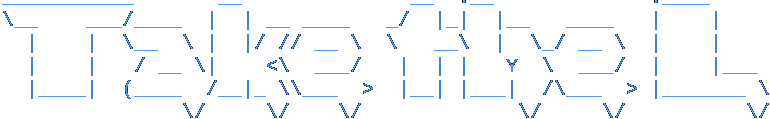
\includegraphics[scale=0.3]{logo.png} \\ \textbf{First Practical Assignment}}
\author{Artifical Intelligence \\ Bachelors in Informatics and Computer Engineering \\ \\ Group 14\_1C   \\ Mário Travassos up201905871@up.pt \\ Rita Mendes up201907877@up.pt \\ Tiago Rodrigues up201907021@up.pt }

\graphicspath{{./images/}}

\begin{document}

    \maketitle

    \newpage

     \section{Introduction}

     \paragraph{}The assigned project consists in the attempt to develop a solitaire game, called "[Exactly One Mazes](https://erich-friedman.github.io/puzzle/exactly1/)", along with the development of an algorithm that can solve the game at different levels, using different heuristics and search methods as basis of work.

     \paragraph{}Then, the algorithms should be compared, in order to find the most efficient one, factoring in terms like speed of execution, memory usage, amount of operations performed, etc.

     \paragraph{}The game will be developed with a graphical user interface in mind, whilst being mostly keyboard centered. The player will control his actions via the arrow keys, and will use enter to select any option, and backspace to return to the starting point.

     \subsection{Game description}

     \paragraph{}In essence, the goal of the game is to find a path that will move horizontally and vertically from the Start in the lower left corner, to the Finish in the upper right one. The challenge is that the path must pass through each L shape at least once, and it cannot go through the same square more than once.

     \subsection{A Formulation as a Search Problem}

     \paragraph{}The problem can be though of as a search problem, attending to the fact that we are trying to find the sequence of states that will lead us to a goal, which is having a path that touches all L shapes at least once, and finishes on the top right corner of the board.

     \paragraph{}\textbf{Complete this after having a better understanding of how things work}

\end{document}
